\documentclass[border=10pt]{standalone}
\usepackage[svgnames]{xcolor}
\usepackage{amsmath}
\usepackage{pgfplots}
\pgfplotsset{compat=newest}
\usepackage[sfdefault]{FiraSans}
\usepackage{FiraMono}
\renewcommand*\familydefault{\sfdefault}
\begin{document}
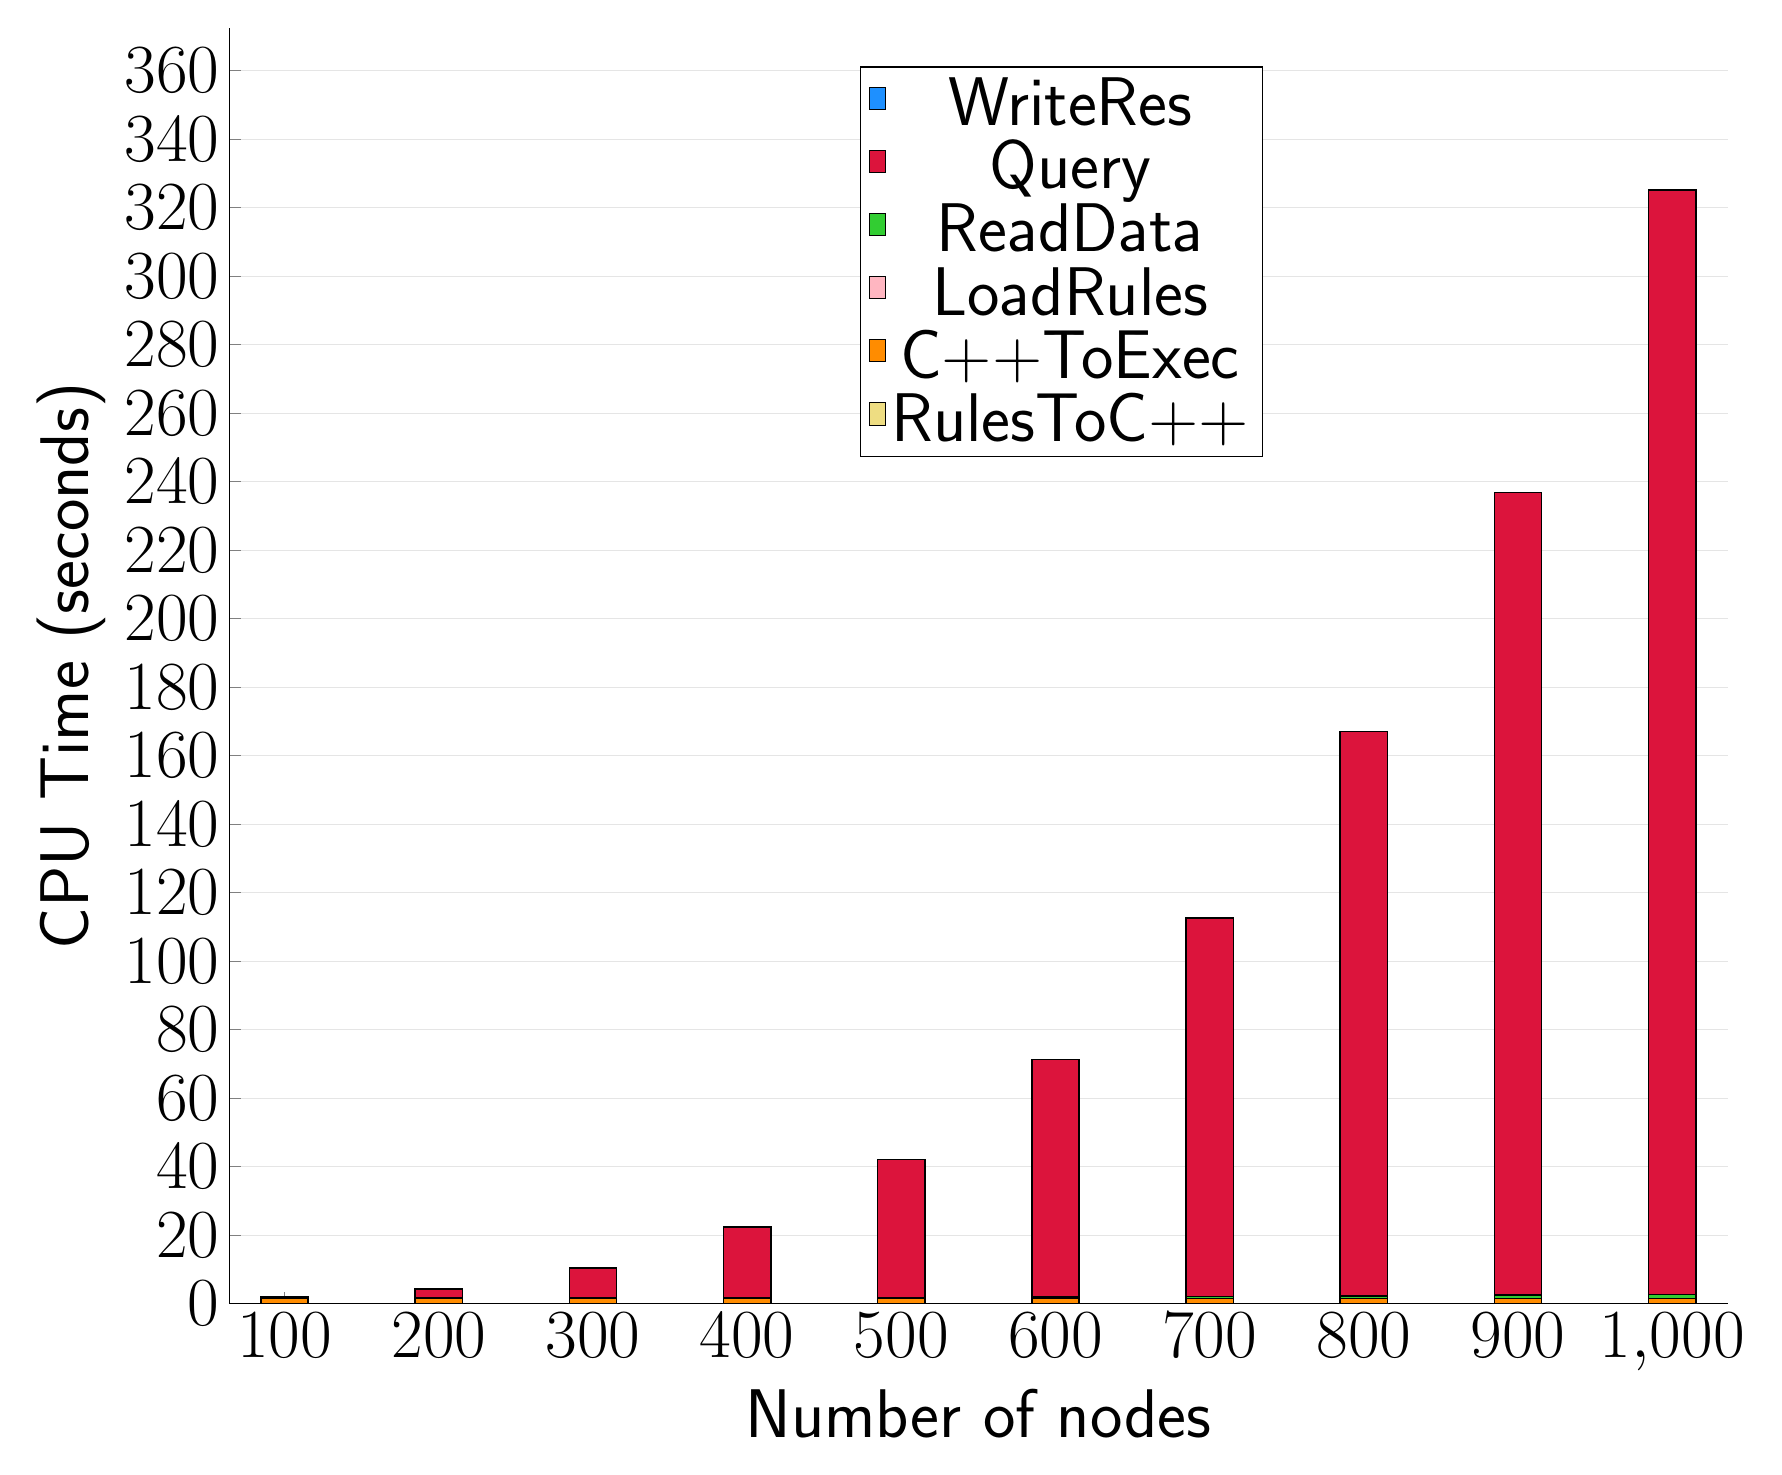
\begin{tikzpicture}
\begin{axis}[
   ybar stacked,
   width=1.7\textwidth,
   bar width=0.6cm,
   ymajorgrids, tick align=inside,
   major grid style={draw=gray!20},
   xtick=data,
   ymin=0, ymax=372.4108,
   axis x line*=bottom,
   axis y line*=left,
   enlarge x limits=0.04,
   legend style={
       at={(0.69, 0.97)},
       anchor=north east,
       legend columns=1,
       font=\Huge,
   },
   ylabel={CPU Time (seconds)},
   xlabel={Number of nodes},
   label style={font=\Huge},
   tick label style={font=\Huge},
]
\addlegendimage{fill=DodgerBlue, draw=black, line width=0.2pt}
\addlegendentry{WriteRes}
\addlegendimage{fill=Crimson, draw=black, line width=0.2pt}
\addlegendentry{Query}
\addlegendimage{fill=LimeGreen, draw=black, line width=0.2pt}
\addlegendentry{ReadData}
\addlegendimage{fill=LightPink, draw=black, line width=0.2pt}
\addlegendentry{LoadRules}
\addlegendimage{fill=DarkOrange, draw=black, line width=0.2pt}
\addlegendentry{C++ToExec}
\addlegendimage{fill=LightGoldenrod, draw=black, line width=0.2pt}
\addlegendentry{RulesToC++}
\addplot +[fill=LightGoldenrod, draw=black, line width=0.55pt] coordinates {
(100, 0.008000000000000002)
(200, 0.010000000000000002)
(300, 0.006000000000000001)
(400, 0.008000000000000002)
(500, 0.008000000000000002)
(600, 0.006000000000000001)
(700, 0.0020000000000000005)
(800, 0.0)
(900, 0.0)
(1000, 0.0)
};
\addplot +[fill=DarkOrange, draw=black, line width=0.55pt] coordinates {
(100, 1.532)
(200, 1.5320000000000003)
(300, 1.538)
(400, 1.544)
(500, 1.53)
(600, 1.536)
(700, 1.534)
(800, 1.5340000000000003)
(900, 1.532)
(1000, 1.536)
};
\addplot +[fill=LightPink, draw=black, line width=0.55pt] coordinates {
(100, 0.000181)
(200, 0.0001506)
(300, 0.0001594)
(400, 0.0001644)
(500, 0.0001652)
(600, 0.000176)
(700, 0.0001744)
(800, 0.0001698)
(900, 0.0001672)
(1000, 0.0001484)
};
\addplot +[fill=LimeGreen, draw=black, line width=0.55pt] coordinates {
(100, 0.0229594)
(200, 0.064892)
(300, 0.12425380000000001)
(400, 0.2056292)
(500, 0.309481)
(600, 0.43872220000000006)
(700, 0.5900622)
(800, 0.7630254000000001)
(900, 0.9621511999999999)
(1000, 1.188628)
};
\addplot +[fill=Crimson, draw=black, line width=0.55pt] coordinates {
(100, 0.3392834)
(200, 2.595226)
(300, 8.689760000000001)
(400, 20.643579999999996)
(500, 40.25768)
(600, 69.31989999999999)
(700, 110.43319999999999)
(800, 164.708)
(900, 234.3094)
(1000, 322.4108)
};
\addplot +[fill=DodgerBlue, draw=black, line width=0.55pt] coordinates {
(100, 0.00023180000000000002)
(200, 0.000372)
(300, 0.0004208)
(400, 0.0003874)
(500, 0.0004168)
(600, 0.0004482)
(700, 0.00043440000000000004)
(800, 0.000414)
(900, 0.0004474)
(1000, 0.0005526)
};
\end{axis}
\end{tikzpicture}

\end{document}
